\section{Procedure}
\label{sec:Durchführung}

\subsection{Alignment}
\label{sec:alignmentSpeckle}
\begin{figure}
    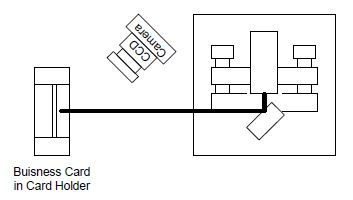
\includegraphics[width=\linewidth]{content/aligment.jpg}
    \caption{Schematic setup for alignment \cite{Anleitung}}
 \end{figure}

The laser diode is placed on an optical breadboard. The same element housing the diode also houses the grating element. Upon heating the laser %word 
An IR viewing card is placed in a cardholder in front of the diode. This card is coated in a polymer which transforms incoming infrared light into visible light.
Additionally, an IR camera is pointed at the viewing card.
Now the current is increased. Soon a light spot will be visible on the card. It will turn brighter with increased current. This is the diode operating as an LED.
With further increase of the current there is a sudden jump in brightness with a speckle pattern in the light spot appearing. This indicates the threshold current was reached, and the diode is now lasing.


\subsection{Observing Rubidium Fluorescence}
\label{sec:DurchRubiFluor}
\begin{figure}
    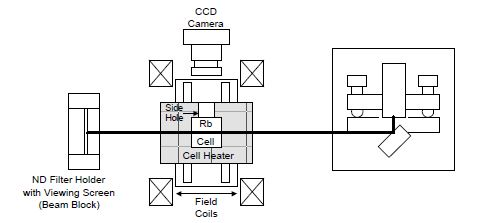
\includegraphics[width=\linewidth]{content/floresence.jpg}
    \caption{Schematic setup for observing rubidium fluorescence.}
 \end{figure}

The viewing card is removed and the laser pass through the rubidium cell. Then a ND filter is positioned behind the cell to prevent stray laser light falling into the room. 
Now the camera is pointed to look into the side of the rubidium cell.  The ramp generator on the control panel is turned on and with the use of an oscilloscope set to an 10 Hz triangle wave.  
The current is adjusted until the fluorescence is observed as a thin flashing line inside the cell.

\begin{figure}
    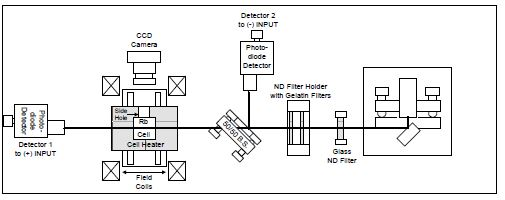
\includegraphics[width=\linewidth]{content/resonance_setup.jpg}
    \caption{Schematic setup for observing rubidium resonance lines.}
 \end{figure}

 For the resonance line, a beam splitter is placed in front of the rubidium cell, directing a part of the beam into a photodetector. Another is placed behind the 
rubidium cell. Some filters must be placed in front of the laser to not saturate the detectors. 
Using the detector electronics on the controller the spectrum of the first detector without the absorption will be subtracted from the other. This results in a clean picture of the absorption spectrum on the oscilloscope. To eliminate mode hops that could distort the spectrum some fine tuning of injection current and grating angle is required.